 % arara: xelatex: {shell: true}
% arara: biber
% arara: xelatex: {shell: true}
% arara: xelatex: {shell: true}

% Podklad k cvičení v předmětu BI-DPR
% autor: Ondřej Guth (ondrej.guth@fit.cvut.cz)
% (c) FIT ČVUT, 2018


\documentclass[a4paper]{article}
\usepackage{polyglossia}
\setmainlanguage{czech}
\usepackage{xevlna,xltxtra}
\usepackage{csquotes}
%\usepackage[style=german]{csquotes} % pro starší verze, kde není čeština

\usepackage[hidelinks]{hyperref}
\usepackage{graphicx}
\usepackage{minted}
\usepackage{xfrac}
\usepackage{nicefrac}
\usepackage[style=iso-numeric]{biblatex}

\title{MI-PAA\\
\large Úkol 2 -- zpráva\\}

\author{Tomáš Přeučil}

\begin{document}

\maketitle

%\tableofcontents

\section{Zadání úlohy}
	Zadáním úlohy bylo naprogramování pokročilých technik pro řešení problému batohu. Konkrétně branch and bound, dynamické programování podle ceny/kapacity a FPTAS algoritmus. Dále pak testování těchto metod.


\section{Použité prostředky}
	\subsection{Programovací jazyky a software}
		Úloha byla řešena v jazyce Python ve verzi 3.6 pod operačním systémem OS X 10.11.6. Program byl spouštěn z Bashe a tudíž pro spuštění nebylo využito žádné IDE.
		Pro měření času byla využita knihovna time a funkce \textit{time.process\_time()}. Jedná se o novinku od verze 3.3, která pracuje velmi podobně jako doporučovaná knihovna \textit{timeit}.
		
	\subsection{Konfigurace testovacího stroje}
		Testování bylo provedeno na MacBooku Pro 13", Early 2011, modelové číslo MC700LL/A. Stroj obsahuje CPU Intel Core i5 2415M (2,3~GHz) a 16~GB RAM. Jediný další rozdíl oproti výchozí konfiguraci je vyměněný disk (za SSD), což však v tomto případě nehraje roli.

\section{Rozbor možných variant řešení, rámcový postup jejich implementace a jejich popis}
	Metodu branch and bound lze naprogramovat dvěma různými způsoby. První je postupné lineární procházení vstupu seřazeného dle poměru cena/váha a stavění stromu s dle přítomnosti věcí v batohu. Tato metoda se snaží procházet tou cestou ve stromě, která vede nejvyššímu potenciálnímu zisku. Toho je dosaženo pomocí prioritní fronty uzlů.
	
	Druhou, na naprogramování značně jednodušší, metodou je rekurzivní zanořování a zaříznutí větve rekurze v případě překročení kapacity batohu, nebo v případě že aktuální řešení nemůže přesáhnout nejlepší již nalezené řešení. K tomu stačí na začátku znát sumu všech hodnot (která je v rekurzivním stromě předávána níže, vždy snížena o hodnotu aktuální věci) a mít jednu globální proměnnou s aktuálním maximem.
	
	Co se dynamického programování týče, je možné volit mezi dekompozicí podle váhy a podle ceny. Obě varianty snižují výpočetní náročnost na úkor náročnosti paměťové a předpočítávají výsledky podproblémů tak, aby žádný z nich nebyl řešen vícekrát.
	
	Pro dekompozici podle ceny stačí vytvořit globální pole o rozměru kapacita x počet věcí. V případě že vypočítáme řešení pro danou kapacitu a danou věc, vložíme ho do pole. Na začátku funkce pak stačí kontrolovat, jestli daný podproblém již nebyl řešen a dle toho se buď zanořit hlouběji, nebo vrátit již spočtené řešení.
	
	U dekompozice podle ceny je nutné vytvořit pole o rozměru počet věcí x všechny možné ceny. To může být obrovský problém při použití desetinných čísel. Zde je tabulku nutné procházet iterativně a následně za posledního sloupce vybrat řešení, což se provede tak, že hledáme nejvyšší index v posledním sloupci, kde kapacita nepřekračuje kapacitu batohu.
	
	Algoritmus FPTAS je rozšířením dynamického programování. Umožňuje škálovat osu udávající cenu výměnou za sníženou přesnost. Při použití celých čísel se může jednat například o vydělení všech cen nějakou konstantou, kterou je výsledek následně přenásoben.

\section{Rámcový popis postupu řešení}
	Idea byla testovat vše z jednoho programu. Pro každou metodu byl tedy vytvořen \enquote{wrapper}, který je volán z hlavního programu.
	
	Byly vytvořeny funkce pro Branch and Bound (zde byla vybrána rekurzivní varianta), dynamické programování dle ceny i kapacity a funkce pro dekompozici dle ceny byla rozšířena o možnost použití algoritmu FPTAS. Všechny funkce byly implementovány přesně dle postupu uvedeného v předchozí sekci.
	
	Z důvodu rozumného měření času byly pro počet věcí menší než 20 volány všechny funkce stokrát a výsledný čas byl stem vydělen.
	
	Následný výstup byl zpracován pomocí awk a LibreOffice.

\section{Naměřené výsledky}
	Nejprve byly naměřeny doby výpočtu pro všechny algoritmy. Ty znázorňuje graf \ref{all-times} s logaritmickým měřítkem. Pro přehlednost jsou data porovnávána i v dalších grafech.
	
	\begin{figure}[h]\centering
		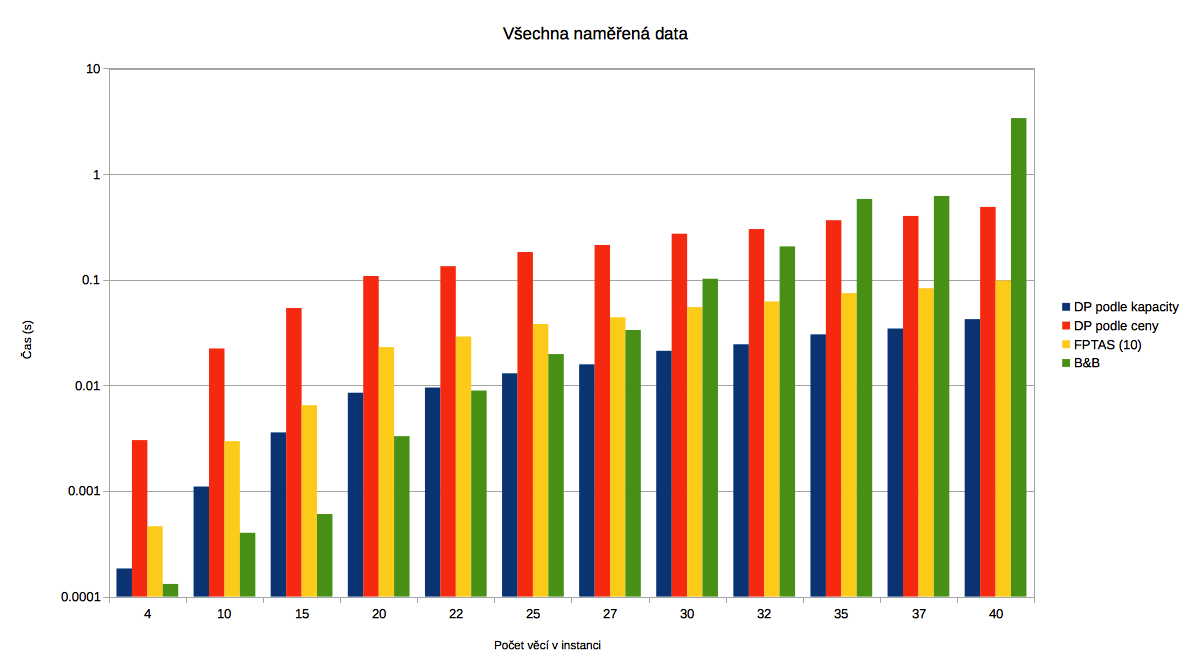
\includegraphics[width=0.99\textwidth]{allData.png} 
		\caption{Časy všech výpočtů}
		\label{all-times}
	\end{figure}
	
	Z detailních porovnání bylo jako první provedeno srovnání různých dekompozic v dynamickém programování s poměrně překvapivými výsledky. Rekurzivní algoritmus dekompozice podle hmotnosti se ukázal jako výrazně rychlejší než iterace při dekompozici dle ceny.  Proto bylo provedeno experimentální měření počtu provedených operací a ukázalo se, že rekurze musí provést výrazně méně průchodů. Například pro instanci 9054 o 10 prvcích jsou hodnoty 554 a 1512 operací. Pro instanci 9035 o 4 prvcích je rozdíl ještě markantnější s 25 a 213 operacemi. Porovnání času je na grafu \ref{dynamic}.
	
	\begin{figure}[h]\centering
		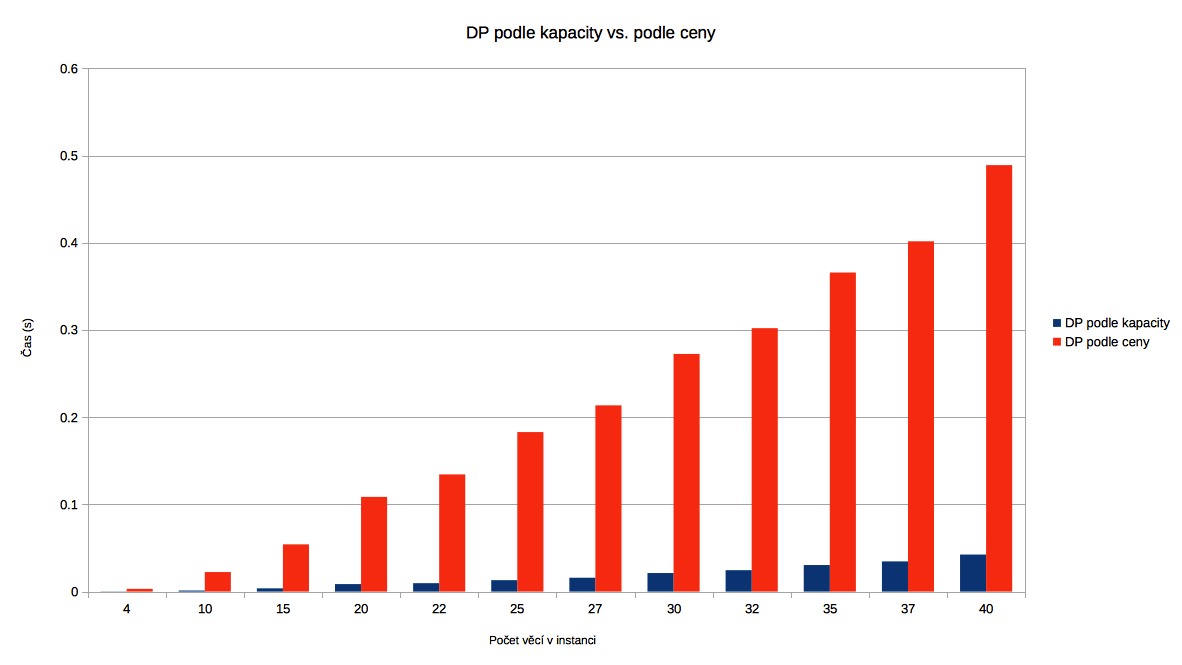
\includegraphics[width=0.99\textwidth]{capVsValue.png}  
		\caption{Srovnání dynamického programován podle kapacity a podle ceny}
		\label{dynamic}
	\end{figure}
	
	Dalším srovnáním je čas výpočtu za pomocí FPTAS algoritmu na základě parametru. Nepřekvapivě se se zvyšující hodnotou časy snižují -- alg. FPTAS výrazně snižuje velikost pole k vyplnění. Tato měření proběhla na instanci o velikosti 40 věcí. Data jsou na grafu \ref{fptas-times}.
	
	\begin{figure}[h]\centering
		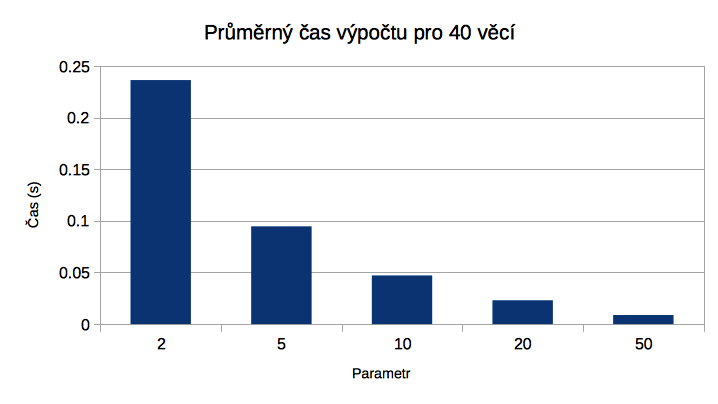
\includegraphics[width=0.99\textwidth]{casyFPTAS.png}  
		\caption{Časy výpočtu FPTAS alg. s ohledem na hodnotu parametru}
		\label{fptas-times}
	\end{figure}
	
	Dále byla srovnána doba výpočtu pro dekompozici dle ceny a FPTAS s hodnotou parametru 10. Měření lze vidět na grafu \ref{fptas-vs-dynamic}. Opět dochází k nepřekvapivému zrychlení, které je cca pětinásobné.
	
	\begin{figure}[h]\centering
		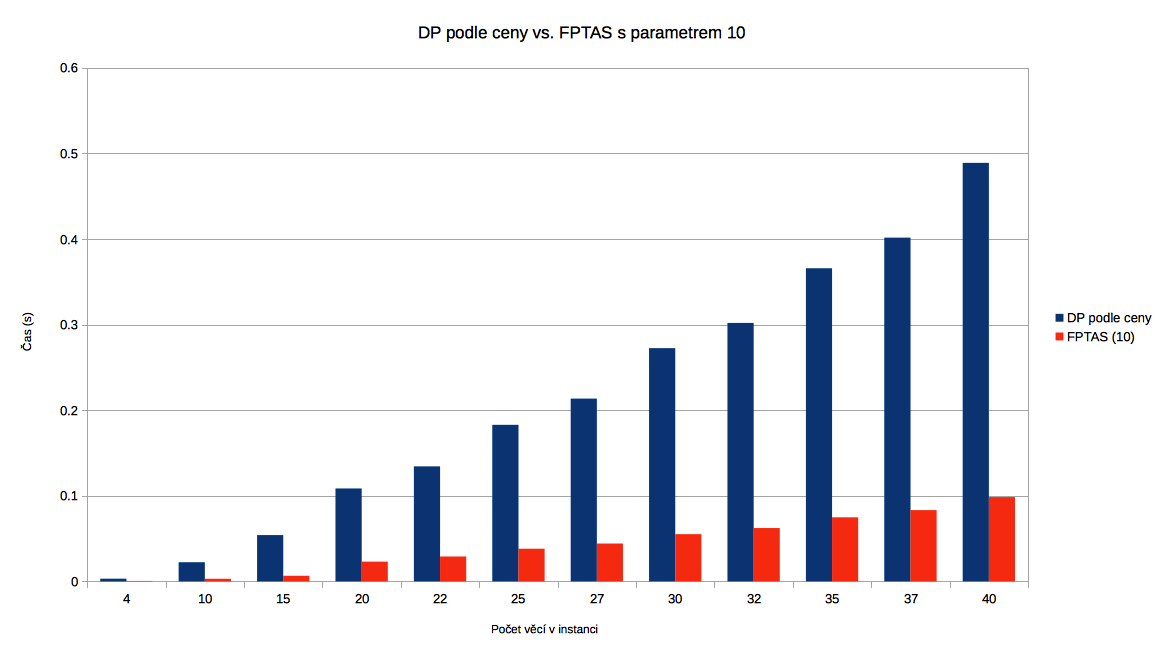
\includegraphics[width=0.99\textwidth]{DPvsFPTAS.png} 
		\caption{Porovnání časů vypočtu pro DP a FPTAS}
		\label{fptas-vs-dynamic}
	\end{figure}
	
	Poslední sledovanou veličinou byla relativní maximální a průměrná chyba. Zde nastalo největší překvapení a zklamání. Maximální chyba je i při vydělení ceny dvěma velmi, \textbf{velmi}, vysoká. To je bohužel dáno obsahem vstupních dat. U vyšších hodnot parametru dokonce maximální chyba dosáhla tak vysoké hodnoty, že algoritmus vůbec nenašel řešení. Je ale nutné dodat, že toto jsou \textbf{mezní případy}. Výskyty takto vysoké chyby jsou ve výstupu velmi ojedinělé. Průměrná chyba toto ukazuje, ačkoli i ta je u vysokých hodnot parametrů daleko od zanedbatelnosti. Měřená data se nachází v příloze a jejich reprezentaci lze najít na grafu \ref{fptas-error}.
	
	Jako poslední by se hodilo říci, že FPTAS je vhodný primárně pro desetinné vstupy (kde při vysoké přesnosti je spotřeba paměti extrémní), nebo pro velmi velká čísla (opět reprezentována jako float).
	
	\begin{figure}[h]\centering
		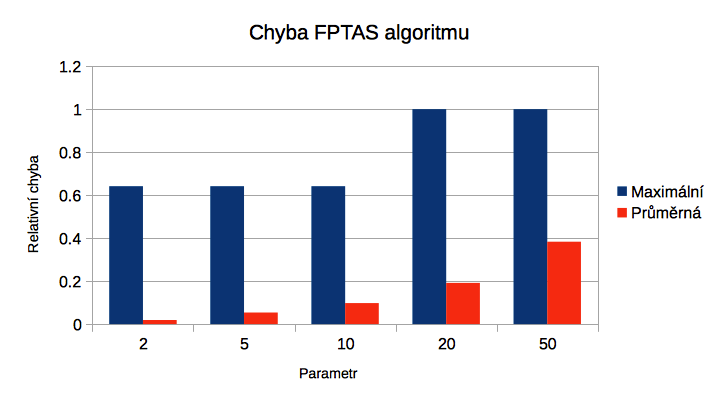
\includegraphics[width=0.99\textwidth]{chybaFPTAS.png} 
		\caption{Chyba FPTAS algoritmu}
		\label{fptas-error}
	\end{figure}
	



\section{Závěr}
	Algortmus Branch and Bound se choval zcela dle očekávání. Sice je i nadále exponenciální (protože se pořád jedná o bruteforce), ale ve srovnání s hrubou sílou je výrazně rychlejší. Dynamické programování nejdříve překvapilo rozdílem mezi rychlostí dekompozice dle ceny a kapacity, ale nakonec se ukázalo, že se jedná pouze o implementační záležitost.
	FPTAS algoritmus zklamal výsledky maximální chyby v momentě, kdy jsou na vstupu celá čísla. V momentě, kdy by na vstupu byla čísla desetinná a docházelo by k zanedbávání desetinných míst, výsledek by jistě byl lepší. Průměrná chyba byla pro nízké hodnoty parametru v přijatelných mezích, ale opět -- mezní případy zde opravdu vadí.
%bab exp, zbytek poly



\end{document}